%Este trabalho está licenciado sob a Licença Atribuição-CompartilhaIgual 4.0 Internacional Creative Commons. Para visualizar uma cópia desta licença, visite http://creativecommons.org/licenses/by-sa/4.0/deed.pt_BR ou mande uma carta para Creative Commons, PO Box 1866, Mountain View, CA 94042, USA.

\chapter{Introdução}\label{cap_intro}

\begin{flushright}
  [Áudio] | [Vídeo] | \href{https://phkonzen.github.io/notas/contato.html}{[Contatar]}
\end{flushright}

Neste capítulo, introduzimos conceitos e definições elementares sobre \emph{equações a diferenças}. Por exemplo, definimos tais equações, apresentamos alguns exemplos de modelagem matemática e problemas relacionados.

\section{Equações a diferenças}\label{cap_intro_sec_ead}

\begin{flushleft}
  [Áudio] | \href{https://archive.org/details/ead-intro}{[Vídeo]} | \href{https://phkonzen.github.io/notas/contato.html}{[Contatar]}
\end{flushleft}

Equações a diferenças são aquelas que podem ser escritas na seguinte forma
\begin{equation}\label{eq:intro_ead}
  f\left(y(n+k),y(n+k-1),\dotsc,y(n);n\right) = 0,
\end{equation}
onde $n=0, 1, 2, \ldots$, $k\geq 0$ número natural e $y:n\mapsto y(n)$ é função discreta (incógnita).

\begin{ex}\label{ex:intro_modelos}
  Vejamos os seguintes exemplos.
  \begin{enumerate}[a)]
  \item \emph{Modelo de juros compostos}
    \begin{equation}
      y(n+1) = (1+r)y(n)
    \end{equation}
    Esta equação a diferenças modela uma aplicação corrigida a juros compostos com taxa $r$ por período de tempo $n$ (dia, mês, ano, etc.). Mais especificamente, seja $y(0)$ o valor da aplicação inicial, então
    \begin{equation}
      y(1) = (1+r)y(0)
    \end{equation}
    é o valor corrigido a taxa $r$ no primeiro período (dia, mês, ano). No segundo período, o valor corrigido é
    \begin{equation}
      y(2) = (1+r)y(1)
    \end{equation}
    e assim por diante.
  \item \emph{Equação logística}
    \begin{equation}
      y(n+1) = r y(n)\left(1 - \frac{y(n)}{K}\right),
    \end{equation}
    onde $y(n)$ representa o tamanho da população no período $n$, $r$ é a taxa de crescimento e $K$ um limiar de saturação.
  \item \emph{Sequência de Fibonacci}\footnote{Fibonacci, c. 1170 - c. 1240, matemático italiano. Fonte: \href{https://en.wikipedia.org/wiki/Fibonacci}{Wikipedia}.}
    \begin{equation}
      y(n+2) = y(n+1) + y(n),
    \end{equation}
    onde $y(0)=1$ e $y(1)=1$.
  \end{enumerate}
\end{ex}

Uma equação a diferenças \eqref{eq:intro_ead} é dita ser de {\bf ordem $k$} (ou de $k$-ésima ordem). É dita ser {\bf linear} quando $f$ é função linear nas variáveis dependentes $y(n+k), y(n+k-1), \dotsc, y(n)$, noutro caso é dita ser {\bf não linear}.

\begin{ex}
  No Exemplo \ref{ex:intro_modelos}, temos
  \begin{enumerate}[a)]
  \item O modelo de juros compostos é dado por equação a diferenças de primeira ordem e linear.
  \item A equação logística é uma equação a diferenças de primeira ordem e não linear.
  \item A sequência equação de Fibonacci é descrita por uma equação a diferenças de segunda ordem e linear.
  \end{enumerate}
\end{ex}

A \emph{solução} de uma equação a diferenças \eqref{eq:intro_ead} é uma sequência de números $\left(y(n)\right)_{n=0}^\infty = \left(y(0), y(1), \dotsc, y(n), \ldots\right)$ que satisfazem a equação.

\begin{ex}\label{ex:ead_intro_ex_solo1}
  Vamos calcular os primeiros quatro valores da solução de
  \begin{align}
    &y(n+1) = 2y(n) - 1,\\
    &y(0)=0.
  \end{align}
  Para tanto, podemos fazer o seguinte procedimento iterativo. Tendo o valor inicial $y(0)=0$, temos
  \begin{align}
    y(1) &= 2y(0) - 1\\
    &= 2\cdot 0 - 1\\
    &= -1.
  \end{align}
  Calculado $y(1)=-1$, temos
  \begin{align}
    y(2) &= 2y(1) - 1\\
    &= 2\cdot (-1) - 1\\
    &= -3.
  \end{align}
  Então, seguimos
  \begin{align}
    y(3) &= 2y(2) - 1\\
    &= 2\cdot (-3) - 1\\
    &= -7.\\
    y(4) &= 2y(3) - 1\\
    &= 2\cdot (-7) - 1\\
    &= -15.
  \end{align}

  Com estes cálculos, podemos concluir que a solução da equação a diferenças é uma sequência da forma
  \begin{equation}
    (y(n))_{n=0}^\infty = (0, -1, -3, -7, -15, \ldots).
  \end{equation}
  Podemos ilustrar a solução conforme feito na figura abaixo.

  \begin{figure}[H]
    \centering
    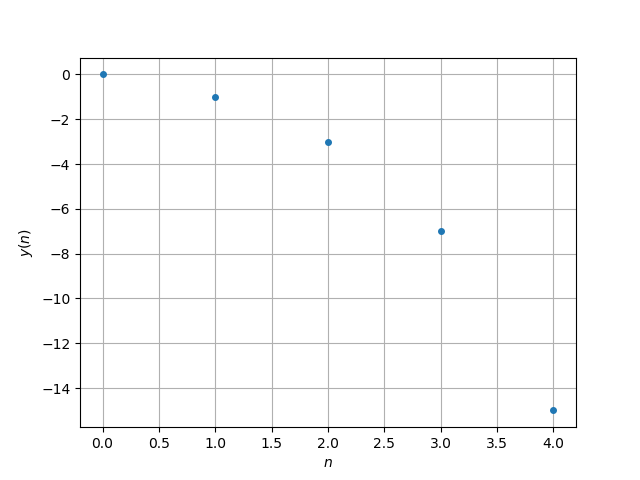
\includegraphics[width=0.7\textwidth]{cap_intro/dados/fig_ead1_intro_ex_solo1/fig.png}
    \caption{Esboço do gráfica da solução da equação a diferenças discutida no Exemplo \ref{ex:ead_intro_ex_solo1}.}
    \label{fig:ead1_intro_ex_solo1}
  \end{figure}
\end{ex}

Para algumas equações a diferenças, é possível escrever a \emph{solução} como uma \emph{forma fechada}
\begin{equation}
  y(n) = g(n),
\end{equation}
onde $n = 0, 1, \ldots$ e $g:n\mapsto g(n)$ é a \emph{função discreta} que representa a solução.

\begin{ex}
  Vamos encontrar a solução para o modelo de juros compostos
  \begin{equation}
    y(n+1) = (1+r)y(n),\quad n\geq 0.
  \end{equation}

  A partir do valor inicial $y(0)$, temos
  \begin{align}
    y(1) &= (1+r)y(0)\\
    y(2) &= (1+r)y(1)\\
    &= (1+r)(1+r)y(0)\\
    &= (1+r)^2y(0) \\
    y(3) &= (1+r)y(2)\\
    &= (1+r)(1+r)^2y(0)\\
    &= (1+r)^3y(0)\\
    &\vdots
  \end{align}
  Com isso, podemos inferir que a solução é dada por
  \begin{equation}
    y(n) = (1+r)^ny(0),
  \end{equation}
  onde o valor inicial $y(0)$ é arbitrário.
\end{ex}

\subsection*{Exercícios resolvidos}

\begin{flushright}
  [Vídeo] | [Áudio] | \href{https://phkonzen.github.io/notas/contato.html}{[Contatar]}
\end{flushright}

\begin{exeresol}
  Calcule $y(10)$, sendo que
  \begin{align}
    y(n+1) = 1,05y(n),\quad n\geq0,
    y(0) = 1000.
  \end{align}
\end{exeresol}
\begin{resol}
  Observamos que
  \begin{align}
    y(1) &= 1,05y(0)\\
    y(2) &= 1,05y(1)\\
    &= 1,05\cdot 1,05y(0) \\
    &= 1,05^2y(0)\\
    y(3) &= 1,05y(2)\\
    &=1,05\cdot 1,05^2y(0)\\
    &= 1,05^3y(0)\\
    &\vdots
  \end{align}
  Com isso, temos que a solução da equação a diferenças é
  \begin{equation}
    y(n) = 1,05^ny(0).
  \end{equation}
  Portanto,
  \begin{align}
    y(10) &= 1,05^{10}y(0) \\
    &= 1,05^{10}\cdot 1000 \\
    &\approx 1628,89.
  \end{align}
\end{resol}

\begin{exeresol}
  Uma semente plantada produz uma flor com uma semente no final do primeiro ano e uma flor com duas sementes no final de cada ano consecutivo. Supondo que cada semente é plantada tão logo é produzida, escreva a equação de diferenças que modela o número de flores $y(n)$ no final do $n$-ésimo ano.
\end{exeresol}
\begin{resol}
  No final do ano $n+2\geq 0$, o número de flores é igual a
  \begin{equation}
    y(n+2) = 2u(n+2) + 3d(n+2),
  \end{equation}
  onde $u(n+2)$ é o número de flores plantadas a um ano e $d(n+2)$ é o número de flores plantas há pelo menos dois anos. Ainda, temos
  \begin{equation}
    u(n+2) = u(n+1) + 2d(n+1)
  \end{equation}
  e
  \begin{equation}
    d(n+2) = u(n+1) + d(n+1).
  \end{equation}
  Com isso, temos
  \begin{align}
    y(n+2) &= 2\left[u(n+1)+2d(n-1)\right] + 3\left[u(n+1)+d(n-1)\right] \\
    &= 2y(n+1) + u(n+1) + d(n+1) \\
    &= 2y(n+1) + \underbrace{u(n) + 2d(n)}_{u(n+1)} + \underbrace{u(n) + d(n)}_{d(n+1)} \\
    &= 2y(n+1) + 2u(n) + 3d(n) \\
    &= 2y(n) + y(n).
  \end{align}
  Desta forma, concluímos que o número de plantas é modelado pela seguinte equação a diferenças de segunda ordem e linear
  \begin{equation}
    y(n+2) = 2y(n+1) + y(n+2).
  \end{equation}
\end{resol}

\subsection*{Exercícios}

\begin{flushright}
  [Vídeo] | [Áudio] | \href{https://phkonzen.github.io/notas/contato.html}{[Contatar]}
\end{flushright}

\begin{exer}
  Classifique as seguintes equações a diferenças quanto a ordem e linearidade.
  \begin{enumerate}[a)]
  \item $\displaystyle y(n+1)-\sqrt{2}y(n) = 1$
  \item $\displaystyle ny(n+1) = y(n)\ln(n+1)$
  \item $\displaystyle y(n) = y(n+1) + 2y(n+2) - 1$
  \item $\displaystyle y(n+1) - \left[1-y(n)\right]\left[1+y(n)\right] = 0$
  \item $\displaystyle y(n+2) = n\sqrt{y(n)}$
  \end{enumerate}
\end{exer}
\begin{resp}
  a) ordem 1, linear; b) ordem 1, linear; c) ordem 2, linear; d) ordem 1, não linear; e) ordem 2, não linear;
\end{resp}

\begin{exer}
  Para cada uma das seguintes equações a diferenças, calcule $y(3)$.
  \begin{enumerate}[a)]
  \item $\displaystyle y(n+1)-\sqrt{2}y(n) = 1,\quad y(0)=1$
  \item $\displaystyle ny(n+1) = y(n)\ln(n+1),\quad y(1)=1$
  \end{enumerate}
\end{exer}
\begin{resp}
  a)~$y(3)=3+3\sqrt{2}$; b)~$y(3)=\frac{1}{2}\ln(2)\ln(3)$
\end{resp}

\begin{exer}
  Para cada uma das seguintes equações a diferenças, calcule $y(4)$.
  \begin{enumerate}[a)]
  \item $\displaystyle y(n) = y(n+1) + 2y(n+2) - 1,\quad y(0)=1, y(1)=0$
  \item $\displaystyle y(n+2) = n\sqrt{y(n)},\quad y(0)=1, y(1)=1$
  \end{enumerate}
\end{exer}
\begin{resp}
  a)~$y(4)=1$; b)~$y(4)=0$
\end{resp}

\begin{exer}
  Encontre a equação a diferenças que modela o saldo devedor anual de uma cliente de cartão de crédito com taxa de juros de 200\% a.a. (ao ano), considerando uma dívida inicial no valor de $y(0)$ reais e que o cartão não está mais em uso.
\end{exer}
\begin{resp}
  $y(n+1) = 3y(n)$.
\end{resp}

\begin{exer}
  Considere uma espécie de seres vivos monogâmicos que após um mês de vida entram na fase reprodutiva. Durante a fase reprodutiva, cada casal produz um novo casal por mês. Desconsiderando outros fatores (por exemplo, mortalidade, perda de fertilidade, etc.), encontre a equação a diferenças que modela o número de casais no $n$-ésimo mês. 
\end{exer}
\begin{resp}
  Sequência de Fibonacci
\end{resp}
